
\section{Rechtslineare Grammatiken}
\begin{frame}{Rechtslineare Grammatiken}
	\begin{Definition}
		Eine Grammatik $G = (N, T, S, P)$ nennt man \textbf{rechtslinear}, wenn bei jeder Produktion auf der rechten Seite \textbf{höchstens ein} Nichtterminalsymbol und dieses nur \textbf{als letztes} Symbol steht.\\
		D. h., alle Produktionen folgen dem Schema $$X \to w \quad \text{oder} \quad X \to wY$$ mit $w \in T^*, \; X,Y \in N$.
	\end{Definition}
\end{frame}

\begin{frame}{Reguläre Sprachen}
	\begin{Satz}
		Für jede formale Sprache $L$ sind die folgenden drei Aussagen äquivalent:
		\begin{itemize}
			\item $L$ kann von einem endlichen Akzeptor erkannt werden.
			\item $L$ kann durch einen regulären Ausdruck beschrieben werden.
			\item $L$ kann von einer rechtslinearen Grammatik erzeugt werden.
		\end{itemize}
	\end{Satz}
	
	Eine solche Sprache nennen wir \textbf{regulär}.
\end{frame}

\begin{frame}{Beispiele für Umwandlungen}
	Siehe Übung 13, WS 15/16
\end{frame}

\begin{frame}{Beispiele}
	$G = (\{X\}, \{\word a, \word b\}, X, P )$ mit 
	$$P = \{X \to \word aX \mid \word{ba}X \mid \word b \mid \varepsilon \}$$
	% Das da ist FALSCH:
	% TODO: Nein, ist es nicht. Es entspricht genau der "Umsetzung" des Automaten
	% Aber das könnte man noch besser herausarbeiten: Automat Tikzen und Zustände umbenennen, G' dann aus Automaten "ablesen"
	%$$P = \{X \to aX \mid bY \mid \varepsilon, Y \to aX \mid bZ \mid \varepsilon, Z \to aZ \mid bZ\}$$ 
	ist eine rechtslineare Grammatik. Die dadurch erzeugte Sprache ist \pause $$L(G) = \set{ w \mid \forall v_1, v_2 \in \{\word a,\word b\}^\ast: w \neq v_1 \word{bb} v_2 },$$ der sie beschreibende reguläre Ausdruck ist \pause $$R =  \rx{(a|ba)*(b|O*)}.  $$ Der Automat dazu sieht so aus:
\end{frame}

\begin{frame}
	\begin{figure}[H]
		\centering
		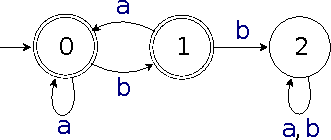
\includegraphics[width=\linewidth]{regulaer/L1.pdf}
	\end{figure}
\end{frame}


\begin{frame}{Achtung!}
	Eine Grammatik kann nicht rechtslinear sein und \textbf{trotzdem} eine reguläre Sprache erzeugen! \\
	\bigskip
	$G = (\set{A}, \set{\word a}, A, \set{A \to \alert{AA} \mid \word a \mid \eps})$, \quad (\alert{nicht} rechtslinear) \\ \pause
	$G' = (\set{A}, \set{\word a}, A, \set{A \to \word aA \mid \eps})$; \quad (rechtslinear) \\ 
	\medskip
	\[\text{und } \quad L(G) = L(G') = \lang{\rx{a*}} \quad \textbf{(regulär!)}\]
\end{frame}

\begin{frame}{Noch mehr Beispiele}
	\begin{itemize}
		\item $G = (\{X \}, \{\word a,\word  b\}, X , \{X \to \word{ab}X \mid \word{bba}X \mid \varepsilon \}$, \\
			$L(G) = \lang{\visible<2-|handout:2>{\rx{(ab|bba)*}}} $
		\item $G = (\{X , Y\}, \{\word a, \word b\}, X , \{X \to \word aX \mid \word bX \mid \word{ababb}Y , Y \to \word aY \mid \word bY \mid \varepsilon \}$, \\
			$L(G) = \lang{\visible<3-|handout:2>{\rx{(a|b)*ababb(a|b)*}}} $
	\end{itemize}
\end{frame}

% Sorry, die Zeit hab ich nicht...
% Ich auch nicht, aber zum Nachlesen lasse ich es trotzdem erstmal drin.
\thasse{
	\begin{frame}{Aufgabe}
		Gegeben ist im folgenden jeweils eine Beschreibung einer formalen Sprache $L$ und ein dazugehöriges Alphabet. Schreiben Sie jeweils den regulären Ausdruck $R$ auf, für den $L(R) = L $ gilt und stellen Sie eine rechtslineare Grammatik $G$ auf, für die $L(G) = L $ gilt:
		\begin{itemize}
			\item Die Menge aller Worte über dem Alphabet $A=\{\word a,\word  b, \word c\}$, die genau ein $\word c$ enthalten. \\
			\visible<2-|handout:2>{
				\emph{Lösung}: $\rx{(a|b)*c(a|b)*}$
			}
			\item Die Menge aller Worte über dem Alphabet $A=\{\word a,\word  b\}$, bei denen die Anzahl der $\word b$ durch 3 teilbar ist. \\
			\visible<3-|handout:2>{
				\emph{Lösung}: $\rx{a*(ba*ba*ba*)*}$
			}
		\end{itemize}
	\end{frame}
	
	\begin{frame}{Aufgabe}
		\textit{Gegeben sei die rechtslineare Grammatik } $$ G= (\{S\},\{\word a,\word  b\},S,P) \qquad P = \{S\to \word{baa}S \mid \word{ba}S \mid \word{aa}S \mid \varepsilon \} $$
		\begin{itemize}
			\only<1-3|handout:1,2>{
				\item Geben Sie einen endlichen Akzeptor $A$ an, so dass $L(A) = L(G)$ gilt
				\only<3|handout:2>{
					\begin{figure}[H]
						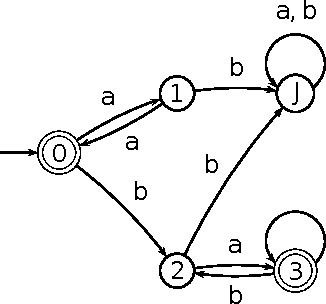
\includegraphics[scale=0.9]{regulaer/L2.pdf}
					\end{figure}
				}
			}
			\only<1,4-5|handout:1,3>{
				\item Gebt einen regulären Ausdruck $R$ an, so dass $ \lang{R} = L(G) $ gilt
				\only<5|handout:3>{
					$$ \rx{(baa|ba|aa)*}$$
				}
			}
			\only<1,6-7|handout:1,3>{
				\item Gebt einen regulären Ausdruck $R$ an, der nicht das Zeichen $\rx{|}$ enthält, und für den $\lang{R}= L(G) $ gilt.
				\only<7|handout:3>{
					$$ \rx{(aa)* (baa*)*} $$
				}
			}
		\end{itemize}
	\end{frame}
	
}



%\begin{frame}
%	\frametitle{Was wir können:}
%	Von..
%	\begin{description}
%		\item[..rechtslinearen Gammatiken..] zu
%		\begin{itemize}
%			\item den Akzeptoren: \pause (mind.) jedes Nichtterminalsymbol ein Zustand, $|$ ist Verzweigung, Akzeptierende Zustände wählen \pause
%			\item den regulären Ausdrücken: \pause Schwierig!
%		\end{itemize}
%		\item[..endlichen Akzeptoren..]  zu
%		\begin{itemize}
%			\item den Grammatiken: \pause Zustandsübergang ist eine Produktion\pause
%			\item den regulären Ausdrücken: \pause Einzelne Wege abgehen
%		\end{itemize}
%		\item[..regulären Ausdrücken..] zu
%		\begin{itemize}
%			\item den Akzeptoren: \pause in Abschnitte teilen, $\ast$ ist Schleife, $|$ ist Verzweigung \pause
%			\item den rechtslinearen Grammatiken: \pause genauso wie Akzeptor
%		\end{itemize}
%	\end{description}
%\end{frame}